% Options for packages loaded elsewhere
\PassOptionsToPackage{unicode}{hyperref}
\PassOptionsToPackage{hyphens}{url}
%
\documentclass[
]{article}
\usepackage{amsmath,amssymb}
\usepackage{iftex}
\ifPDFTeX
  \usepackage[T1]{fontenc}
  \usepackage[utf8]{inputenc}
  \usepackage{textcomp} % provide euro and other symbols
\else % if luatex or xetex
  \usepackage{unicode-math} % this also loads fontspec
  \defaultfontfeatures{Scale=MatchLowercase}
  \defaultfontfeatures[\rmfamily]{Ligatures=TeX,Scale=1}
\fi
\usepackage{lmodern}
\ifPDFTeX\else
  % xetex/luatex font selection
\fi
% Use upquote if available, for straight quotes in verbatim environments
\IfFileExists{upquote.sty}{\usepackage{upquote}}{}
\IfFileExists{microtype.sty}{% use microtype if available
  \usepackage[]{microtype}
  \UseMicrotypeSet[protrusion]{basicmath} % disable protrusion for tt fonts
}{}
\makeatletter
\@ifundefined{KOMAClassName}{% if non-KOMA class
  \IfFileExists{parskip.sty}{%
    \usepackage{parskip}
  }{% else
    \setlength{\parindent}{0pt}
    \setlength{\parskip}{6pt plus 2pt minus 1pt}}
}{% if KOMA class
  \KOMAoptions{parskip=half}}
\makeatother
\usepackage{xcolor}
\usepackage[margin=1in]{geometry}
\usepackage{color}
\usepackage{fancyvrb}
\newcommand{\VerbBar}{|}
\newcommand{\VERB}{\Verb[commandchars=\\\{\}]}
\DefineVerbatimEnvironment{Highlighting}{Verbatim}{commandchars=\\\{\}}
% Add ',fontsize=\small' for more characters per line
\usepackage{framed}
\definecolor{shadecolor}{RGB}{248,248,248}
\newenvironment{Shaded}{\begin{snugshade}}{\end{snugshade}}
\newcommand{\AlertTok}[1]{\textcolor[rgb]{0.94,0.16,0.16}{#1}}
\newcommand{\AnnotationTok}[1]{\textcolor[rgb]{0.56,0.35,0.01}{\textbf{\textit{#1}}}}
\newcommand{\AttributeTok}[1]{\textcolor[rgb]{0.13,0.29,0.53}{#1}}
\newcommand{\BaseNTok}[1]{\textcolor[rgb]{0.00,0.00,0.81}{#1}}
\newcommand{\BuiltInTok}[1]{#1}
\newcommand{\CharTok}[1]{\textcolor[rgb]{0.31,0.60,0.02}{#1}}
\newcommand{\CommentTok}[1]{\textcolor[rgb]{0.56,0.35,0.01}{\textit{#1}}}
\newcommand{\CommentVarTok}[1]{\textcolor[rgb]{0.56,0.35,0.01}{\textbf{\textit{#1}}}}
\newcommand{\ConstantTok}[1]{\textcolor[rgb]{0.56,0.35,0.01}{#1}}
\newcommand{\ControlFlowTok}[1]{\textcolor[rgb]{0.13,0.29,0.53}{\textbf{#1}}}
\newcommand{\DataTypeTok}[1]{\textcolor[rgb]{0.13,0.29,0.53}{#1}}
\newcommand{\DecValTok}[1]{\textcolor[rgb]{0.00,0.00,0.81}{#1}}
\newcommand{\DocumentationTok}[1]{\textcolor[rgb]{0.56,0.35,0.01}{\textbf{\textit{#1}}}}
\newcommand{\ErrorTok}[1]{\textcolor[rgb]{0.64,0.00,0.00}{\textbf{#1}}}
\newcommand{\ExtensionTok}[1]{#1}
\newcommand{\FloatTok}[1]{\textcolor[rgb]{0.00,0.00,0.81}{#1}}
\newcommand{\FunctionTok}[1]{\textcolor[rgb]{0.13,0.29,0.53}{\textbf{#1}}}
\newcommand{\ImportTok}[1]{#1}
\newcommand{\InformationTok}[1]{\textcolor[rgb]{0.56,0.35,0.01}{\textbf{\textit{#1}}}}
\newcommand{\KeywordTok}[1]{\textcolor[rgb]{0.13,0.29,0.53}{\textbf{#1}}}
\newcommand{\NormalTok}[1]{#1}
\newcommand{\OperatorTok}[1]{\textcolor[rgb]{0.81,0.36,0.00}{\textbf{#1}}}
\newcommand{\OtherTok}[1]{\textcolor[rgb]{0.56,0.35,0.01}{#1}}
\newcommand{\PreprocessorTok}[1]{\textcolor[rgb]{0.56,0.35,0.01}{\textit{#1}}}
\newcommand{\RegionMarkerTok}[1]{#1}
\newcommand{\SpecialCharTok}[1]{\textcolor[rgb]{0.81,0.36,0.00}{\textbf{#1}}}
\newcommand{\SpecialStringTok}[1]{\textcolor[rgb]{0.31,0.60,0.02}{#1}}
\newcommand{\StringTok}[1]{\textcolor[rgb]{0.31,0.60,0.02}{#1}}
\newcommand{\VariableTok}[1]{\textcolor[rgb]{0.00,0.00,0.00}{#1}}
\newcommand{\VerbatimStringTok}[1]{\textcolor[rgb]{0.31,0.60,0.02}{#1}}
\newcommand{\WarningTok}[1]{\textcolor[rgb]{0.56,0.35,0.01}{\textbf{\textit{#1}}}}
\usepackage{graphicx}
\makeatletter
\def\maxwidth{\ifdim\Gin@nat@width>\linewidth\linewidth\else\Gin@nat@width\fi}
\def\maxheight{\ifdim\Gin@nat@height>\textheight\textheight\else\Gin@nat@height\fi}
\makeatother
% Scale images if necessary, so that they will not overflow the page
% margins by default, and it is still possible to overwrite the defaults
% using explicit options in \includegraphics[width, height, ...]{}
\setkeys{Gin}{width=\maxwidth,height=\maxheight,keepaspectratio}
% Set default figure placement to htbp
\makeatletter
\def\fps@figure{htbp}
\makeatother
\setlength{\emergencystretch}{3em} % prevent overfull lines
\providecommand{\tightlist}{%
  \setlength{\itemsep}{0pt}\setlength{\parskip}{0pt}}
\setcounter{secnumdepth}{5}
\usepackage{booktabs}
\usepackage{longtable}
\usepackage{array}
\usepackage{multirow}
\usepackage[table]{xcolor}
\usepackage{float}
\usepackage{booktabs}
\usepackage{longtable}
\usepackage{array}
\usepackage{multirow}
\usepackage{wrapfig}
\usepackage{float}
\usepackage{colortbl}
\usepackage{pdflscape}
\usepackage{tabu}
\usepackage{threeparttable}
\usepackage{threeparttablex}
\usepackage[normalem]{ulem}
\usepackage{makecell}
\usepackage{xcolor}
\ifLuaTeX
  \usepackage{selnolig}  % disable illegal ligatures
\fi
\usepackage{bookmark}
\IfFileExists{xurl.sty}{\usepackage{xurl}}{} % add URL line breaks if available
\urlstyle{same}
\hypersetup{
  pdftitle={Impact of PM2.5 Exposure on Low Birth Weight in Ulaanbaatar (2016--2025)},
  pdfauthor={Ahmedi, Barua, Bhuyan, Karayel},
  hidelinks,
  pdfcreator={LaTeX via pandoc}}

\title{Impact of PM2.5 Exposure on Low Birth Weight in Ulaanbaatar
(2016--2025)}
\author{Ahmedi, Barua, Bhuyan, Karayel}
\date{2025-04-29}

\begin{document}
\maketitle

{
\setcounter{tocdepth}{2}
\tableofcontents
}
\begin{Shaded}
\begin{Highlighting}[]
\NormalTok{knitr}\SpecialCharTok{::}\NormalTok{opts\_knit}\SpecialCharTok{$}\FunctionTok{set}\NormalTok{(}\AttributeTok{root.dir =}\NormalTok{ here}\SpecialCharTok{::}\FunctionTok{here}\NormalTok{())}
\end{Highlighting}
\end{Shaded}

\section{1. Load and Clean Data}\label{load-and-clean-data}

\begin{Shaded}
\begin{Highlighting}[]
\CommentTok{\# Read birth weight and live births data}
\NormalTok{birth\_weight\_low }\OtherTok{\textless{}{-}} \FunctionTok{read.csv}\NormalTok{(}\FunctionTok{here}\NormalTok{(}\StringTok{"Data/Raw/BIRTH WEIGTH LOWER THAN 2500 GRAMS.csv"}\NormalTok{), }\AttributeTok{stringsAsFactors =} \ConstantTok{TRUE}\NormalTok{)}

\NormalTok{live\_births }\OtherTok{\textless{}{-}} \FunctionTok{read.csv}\NormalTok{(}\FunctionTok{here}\NormalTok{(}\StringTok{"./Data/Raw/LIVE BIRTHS.csv"}\NormalTok{), }\AttributeTok{stringsAsFactors =} \ConstantTok{TRUE}\NormalTok{)}

\CommentTok{\# Clean live births: remove commas (if any) and converting to numeric()}
\CommentTok{\# Might not need this as a visula check}

\NormalTok{live\_births\_clean }\OtherTok{\textless{}{-}}\NormalTok{ live\_births}
 
 \ControlFlowTok{for}\NormalTok{ (col }\ControlFlowTok{in} \FunctionTok{names}\NormalTok{(live\_births\_clean)[}\SpecialCharTok{{-}}\DecValTok{1}\NormalTok{]) \{}
\NormalTok{   live\_births\_clean[[col]] }\OtherTok{\textless{}{-}} \FunctionTok{as.numeric}\NormalTok{(}\FunctionTok{gsub}\NormalTok{(}\StringTok{","}\NormalTok{, }\StringTok{""}\NormalTok{, live\_births\_clean[[col]]))}
\NormalTok{ \}}

\CommentTok{\# The data is wide, need to convert the data to long format}
\NormalTok{birth\_weight\_low\_long }\OtherTok{\textless{}{-}}\NormalTok{ birth\_weight\_low }\SpecialCharTok{\%\textgreater{}\%} 
  \FunctionTok{pivot\_longer}\NormalTok{(}\SpecialCharTok{{-}}\NormalTok{Aimag, }
               \AttributeTok{names\_to =} \StringTok{"Month"}\NormalTok{, }
               \AttributeTok{values\_to =} \StringTok{"Low\_Birth\_Weight"}\NormalTok{)}

\NormalTok{live\_births\_long }\OtherTok{\textless{}{-}}\NormalTok{ live\_births\_clean }\SpecialCharTok{\%\textgreater{}\%} 
  \FunctionTok{pivot\_longer}\NormalTok{(}\SpecialCharTok{{-}}\NormalTok{Aimag, }
               \AttributeTok{names\_to =} \StringTok{"Month"}\NormalTok{, }
               \AttributeTok{values\_to =} \StringTok{"Live\_Births"}\NormalTok{)}

\CommentTok{\# Merge two datasets}
\NormalTok{births\_merged }\OtherTok{\textless{}{-}} \FunctionTok{left\_join}\NormalTok{(birth\_weight\_low\_long,}
\NormalTok{                           live\_births\_long, }
                           \AttributeTok{by =} \FunctionTok{c}\NormalTok{(}\StringTok{"Aimag"}\NormalTok{, }\StringTok{"Month"}\NormalTok{))}
\CommentTok{\# Removing "X" from month names}
\NormalTok{birth\_weight\_low\_long }\OtherTok{\textless{}{-}}\NormalTok{ birth\_weight\_low\_long }\SpecialCharTok{\%\textgreater{}\%}
  \FunctionTok{mutate}\NormalTok{(}\AttributeTok{Month =} \FunctionTok{gsub}\NormalTok{(}\StringTok{"\^{}X"}\NormalTok{, }\StringTok{""}\NormalTok{, Month))}

\NormalTok{live\_births\_long }\OtherTok{\textless{}{-}}\NormalTok{ live\_births\_long }\SpecialCharTok{\%\textgreater{}\%}
  \FunctionTok{mutate}\NormalTok{(}\AttributeTok{Month =} \FunctionTok{gsub}\NormalTok{(}\StringTok{"\^{}X"}\NormalTok{, }\StringTok{""}\NormalTok{, Month))}

\CommentTok{\# Merging two datasets}
\NormalTok{births\_merged }\OtherTok{\textless{}{-}} \FunctionTok{left\_join}\NormalTok{(birth\_weight\_low\_long, live\_births\_long, }\AttributeTok{by =} \FunctionTok{c}\NormalTok{(}\StringTok{"Aimag"}\NormalTok{, }\StringTok{"Month"}\NormalTok{))}

\CommentTok{\# Creating Date column}
\NormalTok{births\_merged }\OtherTok{\textless{}{-}}\NormalTok{ births\_merged }\SpecialCharTok{\%\textgreater{}\%}
  \FunctionTok{mutate}\NormalTok{(}\AttributeTok{Date =} \FunctionTok{ym}\NormalTok{(Month)) }\SpecialCharTok{\%\textgreater{}\%}
  \FunctionTok{select}\NormalTok{(Aimag, Date, Low\_Birth\_Weight, Live\_Births)}

\CommentTok{\# \# Quick checks}
\CommentTok{\# str(births\_merged)}
\CommentTok{\# colSums(is.na(births\_merged))}
\CommentTok{\# summary(births\_merged)}
\CommentTok{\# class(births\_merged)}
\end{Highlighting}
\end{Shaded}

\begin{Shaded}
\begin{Highlighting}[]
\CommentTok{\# 1. Read and Combine All PM2.5 Files}
\NormalTok{years }\OtherTok{\textless{}{-}} \DecValTok{2015}\SpecialCharTok{:}\DecValTok{2025}
\NormalTok{pm25\_files }\OtherTok{\textless{}{-}} \FunctionTok{paste0}\NormalTok{(}
  \FunctionTok{here}\NormalTok{(}\StringTok{"Data"}\NormalTok{,}\StringTok{"Raw"}\NormalTok{), }
  \StringTok{"/Ulaanbaatar\_PM2.5\_"}\NormalTok{, years, }\StringTok{"\_YTD.csv"}
\NormalTok{)}

\FunctionTok{names}\NormalTok{(pm25\_files) }\OtherTok{\textless{}{-}}\NormalTok{ years}

\CommentTok{\# Read and bind all}
\NormalTok{pm25\_all }\OtherTok{\textless{}{-}} \FunctionTok{map\_dfr}\NormalTok{(pm25\_files, read\_csv, }\AttributeTok{show\_col\_types =} \ConstantTok{FALSE}\NormalTok{)}


\CommentTok{\# 2. Convert all {-}999 to NA across numeric columns only}
\NormalTok{pm25\_all }\OtherTok{\textless{}{-}}\NormalTok{ pm25\_all }\SpecialCharTok{\%\textgreater{}\%}
  \FunctionTok{mutate}\NormalTok{(}\FunctionTok{across}\NormalTok{(}\FunctionTok{where}\NormalTok{(is.numeric), }\SpecialCharTok{\textasciitilde{}} \FunctionTok{na\_if}\NormalTok{(., }\SpecialCharTok{{-}}\DecValTok{999}\NormalTok{)))}


\CommentTok{\# Now I need to convert all the hourly, daily, monthly and yearly data into a DateTime object. The plan is to separate hourly data and take average of hours to make it daily and same to make it monthly. }

\NormalTok{pm25\_all }\OtherTok{\textless{}{-}}\NormalTok{ pm25\_all }\SpecialCharTok{\%\textgreater{}\%}
  \FunctionTok{clean\_names}\NormalTok{() }\CommentTok{\# Date(LT) was giving all troubles. used janitor package to rename to clean                      variable name. it cleaned all the variables name}

\NormalTok{pm25\_all }\OtherTok{\textless{}{-}}\NormalTok{ pm25\_all }\SpecialCharTok{\%\textgreater{}\%}
  \FunctionTok{rename}\NormalTok{(}\AttributeTok{DateTime =}\NormalTok{ date\_lt) }\SpecialCharTok{\%\textgreater{}\%}  
  \FunctionTok{mutate}\NormalTok{(}
    \AttributeTok{DateTime =} \FunctionTok{parse\_date\_time}\NormalTok{(DateTime, }\AttributeTok{orders =} \StringTok{"ymd IMp"}\NormalTok{),}
    \AttributeTok{Date     =} \FunctionTok{date}\NormalTok{(DateTime)}
\NormalTok{  )}

\CommentTok{\# Now I will create 3 dataset, hourly, daily and monthly just to make sure if anything goes wrong I can come back}
\NormalTok{pm25\_hourly }\OtherTok{\textless{}{-}}\NormalTok{ pm25\_all}

\CommentTok{\# DAILY aggregation}
\CommentTok{\# Did not use nowcast as it is smoothed data. used raw concentration}

\NormalTok{pm25\_daily }\OtherTok{\textless{}{-}}\NormalTok{ pm25\_hourly }\SpecialCharTok{\%\textgreater{}\%}
  \FunctionTok{mutate}\NormalTok{(}
    \AttributeTok{Date     =} \FunctionTok{date}\NormalTok{(DateTime)                }\CommentTok{\# extract YYYY{-}MM{-}DD}
\NormalTok{  ) }\SpecialCharTok{\%\textgreater{}\%}
  \FunctionTok{group\_by}\NormalTok{(Date) }\SpecialCharTok{\%\textgreater{}\%}
  \FunctionTok{summarize}\NormalTok{(}
    \AttributeTok{raw\_conc\_daily    =} \FunctionTok{mean}\NormalTok{(raw\_conc, }\AttributeTok{na.rm =} \ConstantTok{TRUE}\NormalTok{),}
    \AttributeTok{aqi\_daily         =} \FunctionTok{mean}\NormalTok{(aqi,      }\AttributeTok{na.rm =} \ConstantTok{TRUE}\NormalTok{),}
    \AttributeTok{hours\_reported    =} \FunctionTok{n}\NormalTok{(),}
    \AttributeTok{hours\_missing\_raw =} \FunctionTok{sum}\NormalTok{(}\FunctionTok{is.na}\NormalTok{(raw\_conc)),}
    \AttributeTok{hours\_missing\_aqi =} \FunctionTok{sum}\NormalTok{(}\FunctionTok{is.na}\NormalTok{(aqi)),}
    \AttributeTok{.groups =} \StringTok{"drop"}
\NormalTok{  ) }\SpecialCharTok{\%\textgreater{}\%}
  \FunctionTok{mutate}\NormalTok{(}
    \AttributeTok{DateTime =} \FunctionTok{as\_datetime}\NormalTok{(Date)             }\CommentTok{\# midnight timestamps}
\NormalTok{  )}

\CommentTok{\# MONTHLY aggregation}
\NormalTok{pm25\_monthly }\OtherTok{\textless{}{-}}\NormalTok{ pm25\_daily }\SpecialCharTok{\%\textgreater{}\%}
  \FunctionTok{mutate}\NormalTok{(}
    \AttributeTok{Month =} \FunctionTok{floor\_date}\NormalTok{(Date, }\StringTok{"month"}\NormalTok{)        }\CommentTok{\# first day of each month}
\NormalTok{  ) }\SpecialCharTok{\%\textgreater{}\%}
  \FunctionTok{group\_by}\NormalTok{(Month) }\SpecialCharTok{\%\textgreater{}\%}
  \FunctionTok{summarize}\NormalTok{(}
    \AttributeTok{raw\_conc\_monthly   =} \FunctionTok{mean}\NormalTok{(raw\_conc\_daily, }\AttributeTok{na.rm =} \ConstantTok{TRUE}\NormalTok{),}
    \AttributeTok{aqi\_monthly        =} \FunctionTok{mean}\NormalTok{(aqi\_daily,      }\AttributeTok{na.rm =} \ConstantTok{TRUE}\NormalTok{),}
    \AttributeTok{days\_reported      =} \FunctionTok{n}\NormalTok{(),}
    \AttributeTok{days\_missing\_raw   =} \FunctionTok{sum}\NormalTok{(}\FunctionTok{is.na}\NormalTok{(raw\_conc\_daily)),}
    \AttributeTok{days\_missing\_aqi   =} \FunctionTok{sum}\NormalTok{(}\FunctionTok{is.na}\NormalTok{(aqi\_daily)),}
    \AttributeTok{.groups =} \StringTok{"drop"}
\NormalTok{  ) }\SpecialCharTok{\%\textgreater{}\%}
  \FunctionTok{mutate}\NormalTok{(}
    \AttributeTok{DateTime =} \FunctionTok{as\_datetime}\NormalTok{(Month)            }\CommentTok{\# first‐of‐month timestamps}
\NormalTok{  )}

\CommentTok{\# YEARLY aggregation}
\NormalTok{pm25\_yearly }\OtherTok{\textless{}{-}}\NormalTok{ pm25\_monthly }\SpecialCharTok{\%\textgreater{}\%}
  \FunctionTok{mutate}\NormalTok{(}
    \AttributeTok{Year =} \FunctionTok{year}\NormalTok{(Month)}
\NormalTok{  ) }\SpecialCharTok{\%\textgreater{}\%}
  \FunctionTok{group\_by}\NormalTok{(Year) }\SpecialCharTok{\%\textgreater{}\%}
  \FunctionTok{summarize}\NormalTok{(}
    \AttributeTok{raw\_conc\_yearly    =} \FunctionTok{mean}\NormalTok{(raw\_conc\_monthly, }\AttributeTok{na.rm =} \ConstantTok{TRUE}\NormalTok{),}
    \AttributeTok{aqi\_yearly         =} \FunctionTok{mean}\NormalTok{(aqi\_monthly,      }\AttributeTok{na.rm =} \ConstantTok{TRUE}\NormalTok{),}
    \AttributeTok{months\_reported    =} \FunctionTok{n}\NormalTok{(),}
    \AttributeTok{months\_missing\_raw =} \FunctionTok{sum}\NormalTok{(days\_missing\_raw }\SpecialCharTok{\textgreater{}} \DecValTok{0}\NormalTok{),}
    \AttributeTok{months\_missing\_aqi =} \FunctionTok{sum}\NormalTok{(days\_missing\_aqi }\SpecialCharTok{\textgreater{}} \DecValTok{0}\NormalTok{),}
    \AttributeTok{.groups =} \StringTok{"drop"}
\NormalTok{  ) }\SpecialCharTok{\%\textgreater{}\%}
  \FunctionTok{mutate}\NormalTok{(}
    \AttributeTok{DateTime =} \FunctionTok{ymd}\NormalTok{(}\FunctionTok{paste0}\NormalTok{(Year, }\StringTok{"{-}01{-}01"}\NormalTok{))    }\CommentTok{\# Jan 1 of each year}
\NormalTok{  )}


\CommentTok{\# Visuallizing pattern}

\FunctionTok{ggplot}\NormalTok{(pm25\_daily, }\FunctionTok{aes}\NormalTok{(}\AttributeTok{x =}\NormalTok{ Date, }\AttributeTok{y =}\NormalTok{ raw\_conc\_daily)) }\SpecialCharTok{+}
  \FunctionTok{geom\_line}\NormalTok{() }\SpecialCharTok{+}
  \FunctionTok{labs}\NormalTok{(}
    \AttributeTok{title =} \StringTok{"Daily PM 2.5 Concentrations (µg/m3)"}\NormalTok{,}
    \AttributeTok{x     =} \StringTok{"Date"}\NormalTok{,}
    \AttributeTok{y     =} \StringTok{"Daily mean raw\_conc"}
\NormalTok{  ) }\SpecialCharTok{+}
  \FunctionTok{theme\_minimal}\NormalTok{()}
\end{Highlighting}
\end{Shaded}

\begin{verbatim}
## Warning: Removed 305 rows containing missing values or values outside the scale range
## (`geom_line()`).
\end{verbatim}

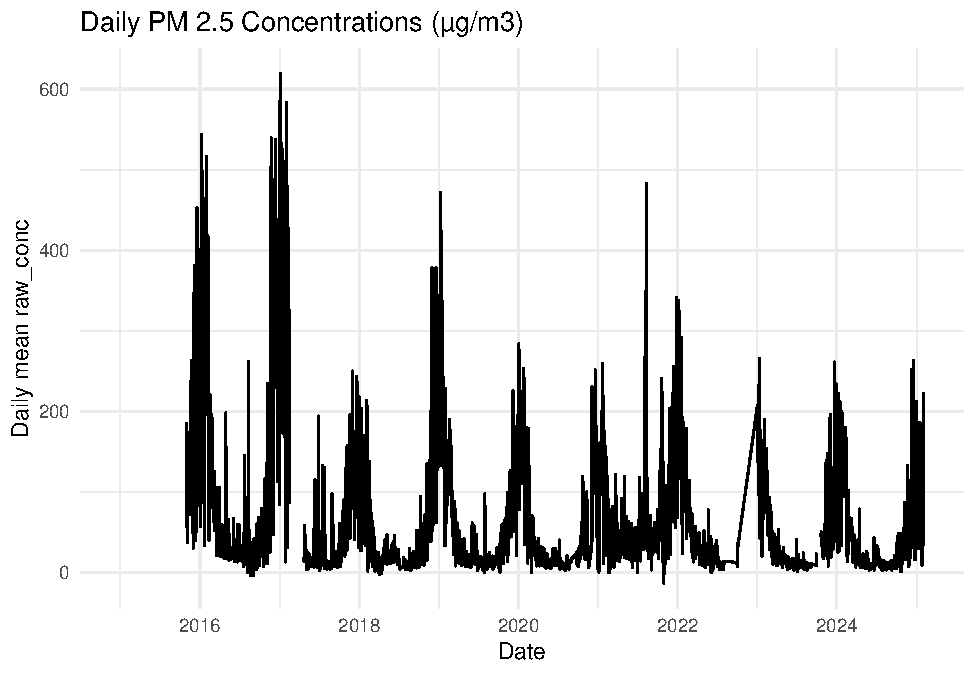
\includegraphics{v_1_files/figure-latex/read-pm25-1.pdf}

\begin{Shaded}
\begin{Highlighting}[]
\CommentTok{\# Treating missing value: }
\CommentTok{\# visualizing missing value}

\CommentTok{\# Bar chart: number of months with ≥1 missing day each year}
\CommentTok{\# Create the pm25\_yearly\_missing summary}
\NormalTok{pm25\_yearly\_missing }\OtherTok{\textless{}{-}}\NormalTok{ pm25\_monthly }\SpecialCharTok{\%\textgreater{}\%}
  \FunctionTok{mutate}\NormalTok{(}\AttributeTok{Year =} \FunctionTok{year}\NormalTok{(Month)) }\SpecialCharTok{\%\textgreater{}\%}
  \FunctionTok{group\_by}\NormalTok{(Year) }\SpecialCharTok{\%\textgreater{}\%}
  \FunctionTok{summarize}\NormalTok{(}
    \AttributeTok{total\_months               =} \FunctionTok{n}\NormalTok{(),}
    \AttributeTok{months\_with\_missing\_days   =} \FunctionTok{sum}\NormalTok{(days\_missing\_raw }\SpecialCharTok{\textgreater{}} \DecValTok{0}\NormalTok{),}
    \AttributeTok{total\_missing\_days         =} \FunctionTok{sum}\NormalTok{(days\_missing\_raw),}
    \AttributeTok{.groups =} \StringTok{"drop"}
\NormalTok{  )}

\CommentTok{\# Plot}
\FunctionTok{ggplot}\NormalTok{(pm25\_yearly\_missing, }\FunctionTok{aes}\NormalTok{(}\AttributeTok{x =}\NormalTok{ Year, }\AttributeTok{y =}\NormalTok{ months\_with\_missing\_days)) }\SpecialCharTok{+}
  \FunctionTok{geom\_col}\NormalTok{(}\AttributeTok{fill =} \StringTok{"tomato"}\NormalTok{) }\SpecialCharTok{+}
  \FunctionTok{labs}\NormalTok{(}
    \AttributeTok{title =} \StringTok{"Number of Months with Missing PM2.5 Data by Year"}\NormalTok{,}
    \AttributeTok{x     =} \StringTok{"Year"}\NormalTok{,}
    \AttributeTok{y     =} \StringTok{"Months with ≥1 Missing Day"}
\NormalTok{  ) }\SpecialCharTok{+}
  \FunctionTok{theme\_minimal}\NormalTok{()}
\end{Highlighting}
\end{Shaded}

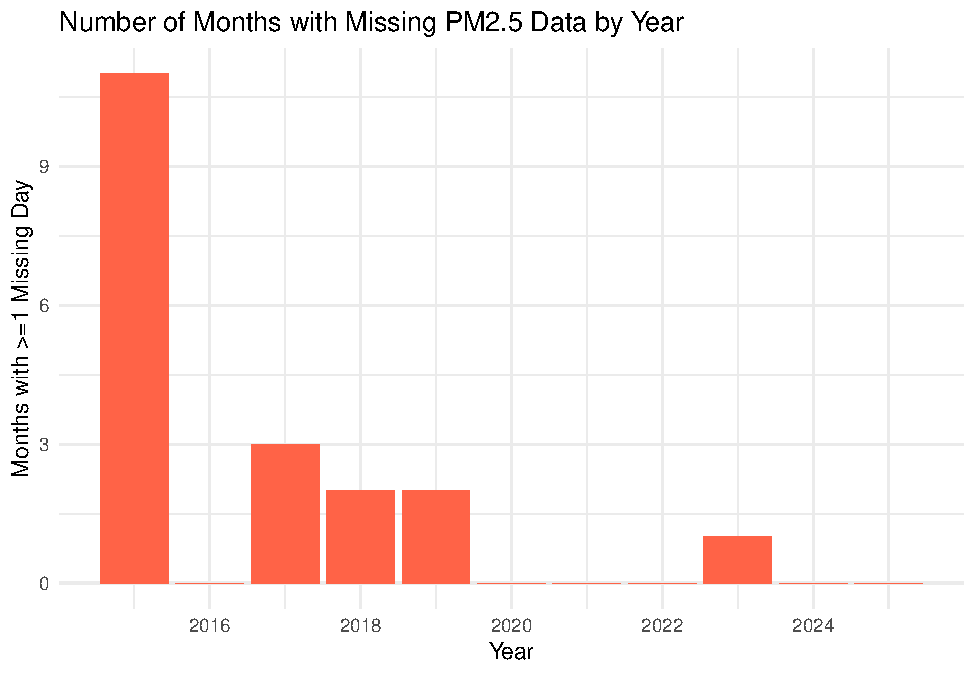
\includegraphics{v_1_files/figure-latex/read-pm25-2.pdf}

\begin{Shaded}
\begin{Highlighting}[]
\CommentTok{\# It looks like there is 9 month of missing data in 2015. We need to consider it afterwards.}

\CommentTok{\# Boxplot of monthly series to spot outliers}
\FunctionTok{ggplot}\NormalTok{(pm25\_monthly, }\FunctionTok{aes}\NormalTok{(}\AttributeTok{y =}\NormalTok{ raw\_conc\_monthly)) }\SpecialCharTok{+}
  \FunctionTok{geom\_boxplot}\NormalTok{(}\AttributeTok{outlier.colour =} \StringTok{"red"}\NormalTok{, }\AttributeTok{outlier.shape =} \DecValTok{1}\NormalTok{) }\SpecialCharTok{+}
  \FunctionTok{labs}\NormalTok{(}
    \AttributeTok{title =} \StringTok{"Distribution of Monthly PM2.5"}\NormalTok{,}
    \AttributeTok{y     =} \StringTok{"Monthly mean PM2.5 (µg/m3)"}
\NormalTok{  ) }\SpecialCharTok{+}
  \FunctionTok{theme\_minimal}\NormalTok{()}
\end{Highlighting}
\end{Shaded}

\begin{verbatim}
## Warning: Removed 11 rows containing non-finite outside the scale range
## (`stat_boxplot()`).
\end{verbatim}

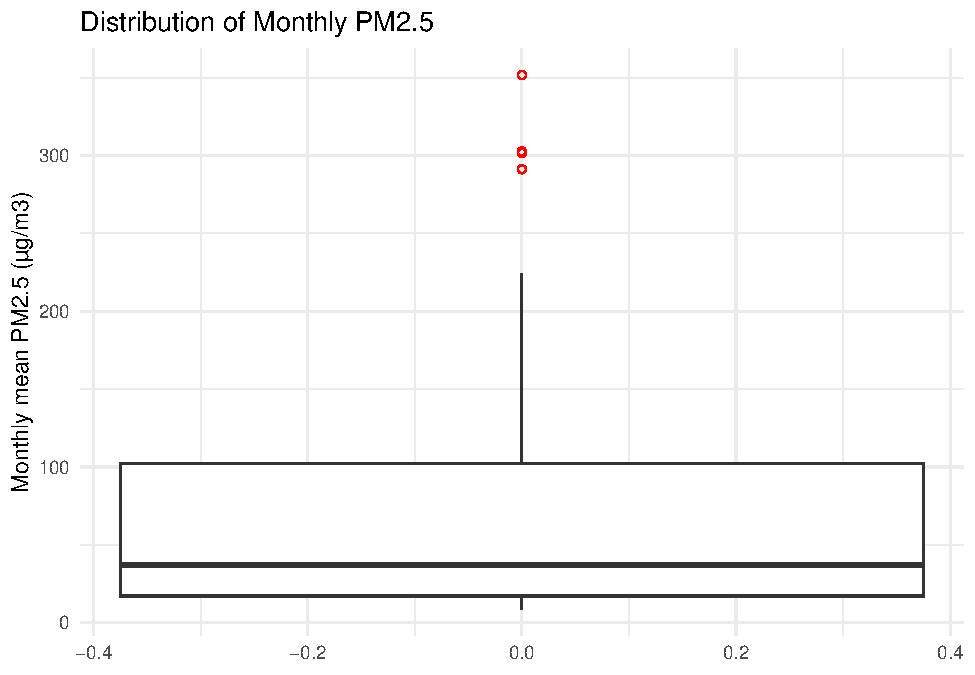
\includegraphics{v_1_files/figure-latex/read-pm25-3.pdf}

\begin{Shaded}
\begin{Highlighting}[]
\CommentTok{\# Looks like does not have a lot of outliers. we can ignore}


\CommentTok{\#write\_csv(pm25\_all, here("Data", "Processed", "pm25\_all.csv"))}



\CommentTok{\# Final NA check}
\FunctionTok{summary}\NormalTok{(pm25\_monthly)}
\end{Highlighting}
\end{Shaded}

\begin{verbatim}
##      Month            raw_conc_monthly   aqi_monthly     days_reported  
##  Min.   :2015-01-01   Min.   :  8.796   Min.   : 31.73   Min.   : 1.00  
##  1st Qu.:2017-06-23   1st Qu.: 17.157   1st Qu.: 55.17   1st Qu.:28.00  
##  Median :2019-12-16   Median : 36.937   Median : 93.02   Median :30.00  
##  Mean   :2019-12-29   Mean   : 69.419   Mean   :114.03   Mean   :28.19  
##  3rd Qu.:2022-06-08   3rd Qu.:102.232   3rd Qu.:173.67   3rd Qu.:31.00  
##  Max.   :2025-02-01   Max.   :351.760   Max.   :274.00   Max.   :31.00  
##                       NA's   :11        NA's   :11                      
##  days_missing_raw days_missing_aqi    DateTime                  
##  Min.   : 0.000   Min.   : 0.000   Min.   :2015-01-01 00:00:00  
##  1st Qu.: 0.000   1st Qu.: 0.000   1st Qu.:2017-06-23 12:00:00  
##  Median : 0.000   Median : 0.000   Median :2019-12-16 12:00:00  
##  Mean   : 3.125   Mean   : 3.225   Mean   :2019-12-29 15:48:00  
##  3rd Qu.: 0.000   3rd Qu.: 0.000   3rd Qu.:2022-06-08 12:00:00  
##  Max.   :31.000   Max.   :31.000   Max.   :2025-02-01 00:00:00  
## 
\end{verbatim}

\begin{Shaded}
\begin{Highlighting}[]
\FunctionTok{colSums}\NormalTok{(}\FunctionTok{is.na}\NormalTok{(pm25\_monthly))}
\end{Highlighting}
\end{Shaded}

\begin{verbatim}
##            Month raw_conc_monthly      aqi_monthly    days_reported 
##                0               11               11                0 
## days_missing_raw days_missing_aqi         DateTime 
##                0                0                0
\end{verbatim}

\begin{Shaded}
\begin{Highlighting}[]
\CommentTok{\# Merge PM2.5 with births}
\NormalTok{full\_data }\OtherTok{\textless{}{-}}\NormalTok{ births\_merged }\SpecialCharTok{\%\textgreater{}\%}
  \FunctionTok{left\_join}\NormalTok{(}
\NormalTok{    pm25\_monthly,}
    \AttributeTok{by =} \FunctionTok{c}\NormalTok{(}\StringTok{"Date"} \OtherTok{=} \StringTok{"Month"}\NormalTok{)}
\NormalTok{  ) }\SpecialCharTok{\%\textgreater{}\%}
  \FunctionTok{arrange}\NormalTok{(Date)}


\NormalTok{full\_data }\SpecialCharTok{\%\textgreater{}\%} 
  \FunctionTok{select}\NormalTok{(Date, Aimag, Low\_Birth\_Weight, Live\_Births, raw\_conc\_monthly, aqi\_monthly)}
\end{Highlighting}
\end{Shaded}

\begin{verbatim}
## # A tibble: 111 x 6
##    Date       Aimag    Low_Birth_Weight Live_Births raw_conc_monthly aqi_monthly
##    <date>     <fct>               <int>       <dbl>            <dbl>       <dbl>
##  1 2016-01-01 Ulaanba~              168        3221            291.        236. 
##  2 2016-02-01 Ulaanba~              152        3158            197.        208. 
##  3 2016-03-01 Ulaanba~              162        3401             73.6       131. 
##  4 2016-04-01 Ulaanba~              132        3229             39.6        87.1
##  5 2016-05-01 Ulaanba~              130        3546             30.5        81.1
##  6 2016-06-01 Ulaanba~              146        3450             29.3        78.4
##  7 2016-07-01 Ulaanba~              179        3696             33.6        77.9
##  8 2016-08-01 Ulaanba~              172        3556             17.2        31.7
##  9 2016-09-01 Ulaanba~              148        3421             22.5        51.5
## 10 2016-10-01 Ulaanba~              159        3566             36.9        83.7
## # i 101 more rows
\end{verbatim}

\begin{Shaded}
\begin{Highlighting}[]
\CommentTok{\# Summary for birth outcomes}
\NormalTok{births\_summary }\OtherTok{\textless{}{-}}\NormalTok{ full\_data }\SpecialCharTok{\%\textgreater{}\%}
  \FunctionTok{summarise}\NormalTok{(}
    \AttributeTok{Mean\_LBW       =} \FunctionTok{mean}\NormalTok{(Low\_Birth\_Weight, }\AttributeTok{na.rm =} \ConstantTok{TRUE}\NormalTok{),}
    \AttributeTok{Median\_LBW     =} \FunctionTok{median}\NormalTok{(Low\_Birth\_Weight, }\AttributeTok{na.rm =} \ConstantTok{TRUE}\NormalTok{),}
    \AttributeTok{Min\_LBW        =} \FunctionTok{min}\NormalTok{(Low\_Birth\_Weight, }\AttributeTok{na.rm =} \ConstantTok{TRUE}\NormalTok{),}
    \AttributeTok{Max\_LBW        =} \FunctionTok{max}\NormalTok{(Low\_Birth\_Weight, }\AttributeTok{na.rm =} \ConstantTok{TRUE}\NormalTok{),}
    \AttributeTok{SD\_LBW         =} \FunctionTok{sd}\NormalTok{(Low\_Birth\_Weight, }\AttributeTok{na.rm =} \ConstantTok{TRUE}\NormalTok{),}
    \AttributeTok{N\_LBW          =} \FunctionTok{sum}\NormalTok{(}\SpecialCharTok{!}\FunctionTok{is.na}\NormalTok{(Low\_Birth\_Weight)),}
    
    \AttributeTok{Mean\_Live      =} \FunctionTok{mean}\NormalTok{(Live\_Births, }\AttributeTok{na.rm =} \ConstantTok{TRUE}\NormalTok{),}
    \AttributeTok{Median\_Live    =} \FunctionTok{median}\NormalTok{(Live\_Births, }\AttributeTok{na.rm =} \ConstantTok{TRUE}\NormalTok{),}
    \AttributeTok{Min\_Live       =} \FunctionTok{min}\NormalTok{(Live\_Births, }\AttributeTok{na.rm =} \ConstantTok{TRUE}\NormalTok{),}
    \AttributeTok{Max\_Live       =} \FunctionTok{max}\NormalTok{(Live\_Births, }\AttributeTok{na.rm =} \ConstantTok{TRUE}\NormalTok{),}
    \AttributeTok{SD\_Live        =} \FunctionTok{sd}\NormalTok{(Live\_Births, }\AttributeTok{na.rm =} \ConstantTok{TRUE}\NormalTok{),}
    \AttributeTok{N\_Live         =} \FunctionTok{sum}\NormalTok{(}\SpecialCharTok{!}\FunctionTok{is.na}\NormalTok{(Live\_Births))}
\NormalTok{  )}

\NormalTok{births\_summary }\SpecialCharTok{\%\textgreater{}\%}
  \FunctionTok{t}\NormalTok{() }\SpecialCharTok{\%\textgreater{}\%} \FunctionTok{as.data.frame}\NormalTok{() }\SpecialCharTok{\%\textgreater{}\%}
  \FunctionTok{rownames\_to\_column}\NormalTok{(}\StringTok{"Statistic"}\NormalTok{) }\SpecialCharTok{\%\textgreater{}\%}
  \FunctionTok{rename}\NormalTok{(}\AttributeTok{Value =}\NormalTok{ V1) }\SpecialCharTok{\%\textgreater{}\%}
  \FunctionTok{kable}\NormalTok{(}\AttributeTok{caption =} \StringTok{"Summary of Birth Outcomes"}\NormalTok{, }\AttributeTok{digits =} \DecValTok{2}\NormalTok{) }\SpecialCharTok{\%\textgreater{}\%}
  \FunctionTok{kable\_styling}\NormalTok{(}\AttributeTok{full\_width =} \ConstantTok{FALSE}\NormalTok{)}
\end{Highlighting}
\end{Shaded}

\begin{verbatim}
## Warning in attr(x, "align"): 'xfun::attr()' is deprecated.
## Use 'xfun::attr2()' instead.
## See help("Deprecated")
\end{verbatim}

\begin{verbatim}
## Warning in attr(.knitEnv$meta, "knit_meta_id"): 'xfun::attr()' is deprecated.
## Use 'xfun::attr2()' instead.
## See help("Deprecated")
## Warning in attr(.knitEnv$meta, "knit_meta_id"): 'xfun::attr()' is deprecated.
## Use 'xfun::attr2()' instead.
## See help("Deprecated")
## Warning in attr(.knitEnv$meta, "knit_meta_id"): 'xfun::attr()' is deprecated.
## Use 'xfun::attr2()' instead.
## See help("Deprecated")
## Warning in attr(.knitEnv$meta, "knit_meta_id"): 'xfun::attr()' is deprecated.
## Use 'xfun::attr2()' instead.
## See help("Deprecated")
## Warning in attr(.knitEnv$meta, "knit_meta_id"): 'xfun::attr()' is deprecated.
## Use 'xfun::attr2()' instead.
## See help("Deprecated")
## Warning in attr(.knitEnv$meta, "knit_meta_id"): 'xfun::attr()' is deprecated.
## Use 'xfun::attr2()' instead.
## See help("Deprecated")
## Warning in attr(.knitEnv$meta, "knit_meta_id"): 'xfun::attr()' is deprecated.
## Use 'xfun::attr2()' instead.
## See help("Deprecated")
## Warning in attr(.knitEnv$meta, "knit_meta_id"): 'xfun::attr()' is deprecated.
## Use 'xfun::attr2()' instead.
## See help("Deprecated")
## Warning in attr(.knitEnv$meta, "knit_meta_id"): 'xfun::attr()' is deprecated.
## Use 'xfun::attr2()' instead.
## See help("Deprecated")
## Warning in attr(.knitEnv$meta, "knit_meta_id"): 'xfun::attr()' is deprecated.
## Use 'xfun::attr2()' instead.
## See help("Deprecated")
## Warning in attr(.knitEnv$meta, "knit_meta_id"): 'xfun::attr()' is deprecated.
## Use 'xfun::attr2()' instead.
## See help("Deprecated")
## Warning in attr(.knitEnv$meta, "knit_meta_id"): 'xfun::attr()' is deprecated.
## Use 'xfun::attr2()' instead.
## See help("Deprecated")
## Warning in attr(.knitEnv$meta, "knit_meta_id"): 'xfun::attr()' is deprecated.
## Use 'xfun::attr2()' instead.
## See help("Deprecated")
## Warning in attr(.knitEnv$meta, "knit_meta_id"): 'xfun::attr()' is deprecated.
## Use 'xfun::attr2()' instead.
## See help("Deprecated")
\end{verbatim}

\begin{verbatim}
## Warning in attr(x, "align"): 'xfun::attr()' is deprecated.
## Use 'xfun::attr2()' instead.
## See help("Deprecated")
\end{verbatim}

\begin{verbatim}
## Warning in attr(x, "format"): 'xfun::attr()' is deprecated.
## Use 'xfun::attr2()' instead.
## See help("Deprecated")
\end{verbatim}

\begin{longtable}[t]{lr}
\caption{\label{tab:Sumamry Staistics}Summary of Birth Outcomes}\\
\toprule
Statistic & Value\\
\midrule
Mean\_LBW & 155.97\\
Median\_LBW & 153.00\\
Min\_LBW & 88.00\\
Max\_LBW & 214.00\\
SD\_LBW & 21.87\\
\addlinespace
N\_LBW & 111.00\\
Mean\_Live & 3110.86\\
Median\_Live & 3187.00\\
Min\_Live & 1934.00\\
Max\_Live & 3737.00\\
\addlinespace
SD\_Live & 360.42\\
N\_Live & 111.00\\
\bottomrule
\end{longtable}

\begin{Shaded}
\begin{Highlighting}[]
\CommentTok{\# 2. Summary for PM2.5 exposure}
\NormalTok{pm25\_summary }\OtherTok{\textless{}{-}}\NormalTok{ full\_data }\SpecialCharTok{\%\textgreater{}\%}
  \FunctionTok{summarise}\NormalTok{(}
    \AttributeTok{Mean\_PM25     =} \FunctionTok{mean}\NormalTok{(raw\_conc\_monthly, }\AttributeTok{na.rm =} \ConstantTok{TRUE}\NormalTok{),}
    \AttributeTok{Median\_PM25   =} \FunctionTok{median}\NormalTok{(raw\_conc\_monthly, }\AttributeTok{na.rm =} \ConstantTok{TRUE}\NormalTok{),}
    \AttributeTok{Min\_PM25      =} \FunctionTok{min}\NormalTok{(raw\_conc\_monthly, }\AttributeTok{na.rm =} \ConstantTok{TRUE}\NormalTok{),}
    \AttributeTok{Max\_PM25      =} \FunctionTok{max}\NormalTok{(raw\_conc\_monthly, }\AttributeTok{na.rm =} \ConstantTok{TRUE}\NormalTok{),}
    \AttributeTok{SD\_PM25       =} \FunctionTok{sd}\NormalTok{(raw\_conc\_monthly, }\AttributeTok{na.rm =} \ConstantTok{TRUE}\NormalTok{),}
    \AttributeTok{N\_PM25        =} \FunctionTok{sum}\NormalTok{(}\SpecialCharTok{!}\FunctionTok{is.na}\NormalTok{(raw\_conc\_monthly)),}

    \AttributeTok{Mean\_AQI      =} \FunctionTok{mean}\NormalTok{(aqi\_monthly, }\AttributeTok{na.rm =} \ConstantTok{TRUE}\NormalTok{),}
    \AttributeTok{Median\_AQI    =} \FunctionTok{median}\NormalTok{(aqi\_monthly, }\AttributeTok{na.rm =} \ConstantTok{TRUE}\NormalTok{),}
    \AttributeTok{Min\_AQI       =} \FunctionTok{min}\NormalTok{(aqi\_monthly, }\AttributeTok{na.rm =} \ConstantTok{TRUE}\NormalTok{),}
    \AttributeTok{Max\_AQI       =} \FunctionTok{max}\NormalTok{(aqi\_monthly, }\AttributeTok{na.rm =} \ConstantTok{TRUE}\NormalTok{),}
    \AttributeTok{SD\_AQI        =} \FunctionTok{sd}\NormalTok{(aqi\_monthly, }\AttributeTok{na.rm =} \ConstantTok{TRUE}\NormalTok{),}
    \AttributeTok{N\_AQI         =} \FunctionTok{sum}\NormalTok{(}\SpecialCharTok{!}\FunctionTok{is.na}\NormalTok{(aqi\_monthly))}
\NormalTok{  )}

\NormalTok{pm25\_summary }\SpecialCharTok{\%\textgreater{}\%}
  \FunctionTok{t}\NormalTok{() }\SpecialCharTok{\%\textgreater{}\%} \FunctionTok{as.data.frame}\NormalTok{() }\SpecialCharTok{\%\textgreater{}\%}
  \FunctionTok{rownames\_to\_column}\NormalTok{(}\StringTok{"Statistic"}\NormalTok{) }\SpecialCharTok{\%\textgreater{}\%}
  \FunctionTok{rename}\NormalTok{(}\AttributeTok{Value =}\NormalTok{ V1) }\SpecialCharTok{\%\textgreater{}\%}
  \FunctionTok{kable}\NormalTok{(}\AttributeTok{caption =} \StringTok{"Summary of Monthly PM2.5 Exposure"}\NormalTok{, }\AttributeTok{digits =} \DecValTok{2}\NormalTok{) }\SpecialCharTok{\%\textgreater{}\%}
  \FunctionTok{kable\_styling}\NormalTok{(}\AttributeTok{full\_width =} \ConstantTok{FALSE}\NormalTok{)}
\end{Highlighting}
\end{Shaded}

\begin{verbatim}
## Warning in attr(x, "align"): 'xfun::attr()' is deprecated.
## Use 'xfun::attr2()' instead.
## See help("Deprecated")
\end{verbatim}

\begin{verbatim}
## Warning in attr(.knitEnv$meta, "knit_meta_id"): 'xfun::attr()' is deprecated.
## Use 'xfun::attr2()' instead.
## See help("Deprecated")
## Warning in attr(.knitEnv$meta, "knit_meta_id"): 'xfun::attr()' is deprecated.
## Use 'xfun::attr2()' instead.
## See help("Deprecated")
## Warning in attr(.knitEnv$meta, "knit_meta_id"): 'xfun::attr()' is deprecated.
## Use 'xfun::attr2()' instead.
## See help("Deprecated")
## Warning in attr(.knitEnv$meta, "knit_meta_id"): 'xfun::attr()' is deprecated.
## Use 'xfun::attr2()' instead.
## See help("Deprecated")
## Warning in attr(.knitEnv$meta, "knit_meta_id"): 'xfun::attr()' is deprecated.
## Use 'xfun::attr2()' instead.
## See help("Deprecated")
## Warning in attr(.knitEnv$meta, "knit_meta_id"): 'xfun::attr()' is deprecated.
## Use 'xfun::attr2()' instead.
## See help("Deprecated")
## Warning in attr(.knitEnv$meta, "knit_meta_id"): 'xfun::attr()' is deprecated.
## Use 'xfun::attr2()' instead.
## See help("Deprecated")
## Warning in attr(.knitEnv$meta, "knit_meta_id"): 'xfun::attr()' is deprecated.
## Use 'xfun::attr2()' instead.
## See help("Deprecated")
## Warning in attr(.knitEnv$meta, "knit_meta_id"): 'xfun::attr()' is deprecated.
## Use 'xfun::attr2()' instead.
## See help("Deprecated")
## Warning in attr(.knitEnv$meta, "knit_meta_id"): 'xfun::attr()' is deprecated.
## Use 'xfun::attr2()' instead.
## See help("Deprecated")
## Warning in attr(.knitEnv$meta, "knit_meta_id"): 'xfun::attr()' is deprecated.
## Use 'xfun::attr2()' instead.
## See help("Deprecated")
## Warning in attr(.knitEnv$meta, "knit_meta_id"): 'xfun::attr()' is deprecated.
## Use 'xfun::attr2()' instead.
## See help("Deprecated")
## Warning in attr(.knitEnv$meta, "knit_meta_id"): 'xfun::attr()' is deprecated.
## Use 'xfun::attr2()' instead.
## See help("Deprecated")
## Warning in attr(.knitEnv$meta, "knit_meta_id"): 'xfun::attr()' is deprecated.
## Use 'xfun::attr2()' instead.
## See help("Deprecated")
\end{verbatim}

\begin{verbatim}
## Warning in attr(x, "align"): 'xfun::attr()' is deprecated.
## Use 'xfun::attr2()' instead.
## See help("Deprecated")
\end{verbatim}

\begin{verbatim}
## Warning in attr(x, "format"): 'xfun::attr()' is deprecated.
## Use 'xfun::attr2()' instead.
## See help("Deprecated")
\end{verbatim}

\begin{longtable}[t]{lr}
\caption{\label{tab:Sumamry Staistics}Summary of Monthly PM2.5 Exposure}\\
\toprule
Statistic & Value\\
\midrule
Mean\_PM25 & 67.28\\
Median\_PM25 & 35.22\\
Min\_PM25 & 8.80\\
Max\_PM25 & 351.76\\
SD\_PM25 & 72.90\\
\addlinespace
N\_PM25 & 107.00\\
Mean\_AQI & 111.86\\
Median\_AQI & 92.67\\
Min\_AQI & 31.73\\
Max\_AQI & 274.00\\
\addlinespace
SD\_AQI & 66.15\\
N\_AQI & 107.00\\
\bottomrule
\end{longtable}

\section{Descriptive Statistics}\label{descriptive-statistics}

\begin{Shaded}
\begin{Highlighting}[]
\CommentTok{\# Compute low birth weight rate (Percentage)}
\NormalTok{full\_data }\OtherTok{\textless{}{-}}\NormalTok{ full\_data }\SpecialCharTok{\%\textgreater{}\%}
  \FunctionTok{mutate}\NormalTok{(}
    \AttributeTok{LBW\_rate =} \DecValTok{100} \SpecialCharTok{*}\NormalTok{ Low\_Birth\_Weight }\SpecialCharTok{/}\NormalTok{ Live\_Births}
\NormalTok{  )}

\CommentTok{\#  Summary table of exposure and outcome}
\NormalTok{summary\_tbl }\OtherTok{\textless{}{-}}\NormalTok{ full\_data }\SpecialCharTok{\%\textgreater{}\%}
  \FunctionTok{summarise}\NormalTok{(}
    \AttributeTok{Mean\_PM25     =} \FunctionTok{mean}\NormalTok{(raw\_conc\_monthly, }\AttributeTok{na.rm =} \ConstantTok{TRUE}\NormalTok{),}
    \AttributeTok{SD\_PM25       =} \FunctionTok{sd}\NormalTok{(raw\_conc\_monthly, }\AttributeTok{na.rm =} \ConstantTok{TRUE}\NormalTok{),}
    \AttributeTok{Mean\_LBWrate  =} \FunctionTok{mean}\NormalTok{(LBW\_rate, }\AttributeTok{na.rm =} \ConstantTok{TRUE}\NormalTok{),}
    \AttributeTok{SD\_LBWrate    =} \FunctionTok{sd}\NormalTok{(LBW\_rate, }\AttributeTok{na.rm =} \ConstantTok{TRUE}\NormalTok{),}
    \AttributeTok{N             =} \FunctionTok{n}\NormalTok{()}
\NormalTok{  ) }\SpecialCharTok{\%\textgreater{}\%}
  \FunctionTok{pivot\_longer}\NormalTok{(}\FunctionTok{everything}\NormalTok{(), }\AttributeTok{names\_to=}\StringTok{"Metric"}\NormalTok{, }\AttributeTok{values\_to=}\StringTok{"Value"}\NormalTok{)}

\NormalTok{summary\_tbl }\SpecialCharTok{\%\textgreater{}\%}
  \FunctionTok{kable}\NormalTok{(}\AttributeTok{caption=}\StringTok{"Summary of PM2.5 and LBW Rate"}\NormalTok{, }\AttributeTok{digits=}\DecValTok{2}\NormalTok{) }\SpecialCharTok{\%\textgreater{}\%}
  \FunctionTok{kable\_styling}\NormalTok{(}\AttributeTok{full\_width=}\ConstantTok{FALSE}\NormalTok{)}
\end{Highlighting}
\end{Shaded}

\begin{verbatim}
## Warning in attr(x, "align"): 'xfun::attr()' is deprecated.
## Use 'xfun::attr2()' instead.
## See help("Deprecated")
\end{verbatim}

\begin{verbatim}
## Warning in attr(.knitEnv$meta, "knit_meta_id"): 'xfun::attr()' is deprecated.
## Use 'xfun::attr2()' instead.
## See help("Deprecated")
## Warning in attr(.knitEnv$meta, "knit_meta_id"): 'xfun::attr()' is deprecated.
## Use 'xfun::attr2()' instead.
## See help("Deprecated")
## Warning in attr(.knitEnv$meta, "knit_meta_id"): 'xfun::attr()' is deprecated.
## Use 'xfun::attr2()' instead.
## See help("Deprecated")
## Warning in attr(.knitEnv$meta, "knit_meta_id"): 'xfun::attr()' is deprecated.
## Use 'xfun::attr2()' instead.
## See help("Deprecated")
## Warning in attr(.knitEnv$meta, "knit_meta_id"): 'xfun::attr()' is deprecated.
## Use 'xfun::attr2()' instead.
## See help("Deprecated")
## Warning in attr(.knitEnv$meta, "knit_meta_id"): 'xfun::attr()' is deprecated.
## Use 'xfun::attr2()' instead.
## See help("Deprecated")
## Warning in attr(.knitEnv$meta, "knit_meta_id"): 'xfun::attr()' is deprecated.
## Use 'xfun::attr2()' instead.
## See help("Deprecated")
## Warning in attr(.knitEnv$meta, "knit_meta_id"): 'xfun::attr()' is deprecated.
## Use 'xfun::attr2()' instead.
## See help("Deprecated")
## Warning in attr(.knitEnv$meta, "knit_meta_id"): 'xfun::attr()' is deprecated.
## Use 'xfun::attr2()' instead.
## See help("Deprecated")
## Warning in attr(.knitEnv$meta, "knit_meta_id"): 'xfun::attr()' is deprecated.
## Use 'xfun::attr2()' instead.
## See help("Deprecated")
## Warning in attr(.knitEnv$meta, "knit_meta_id"): 'xfun::attr()' is deprecated.
## Use 'xfun::attr2()' instead.
## See help("Deprecated")
## Warning in attr(.knitEnv$meta, "knit_meta_id"): 'xfun::attr()' is deprecated.
## Use 'xfun::attr2()' instead.
## See help("Deprecated")
## Warning in attr(.knitEnv$meta, "knit_meta_id"): 'xfun::attr()' is deprecated.
## Use 'xfun::attr2()' instead.
## See help("Deprecated")
## Warning in attr(.knitEnv$meta, "knit_meta_id"): 'xfun::attr()' is deprecated.
## Use 'xfun::attr2()' instead.
## See help("Deprecated")
\end{verbatim}

\begin{verbatim}
## Warning in attr(x, "align"): 'xfun::attr()' is deprecated.
## Use 'xfun::attr2()' instead.
## See help("Deprecated")
\end{verbatim}

\begin{verbatim}
## Warning in attr(x, "format"): 'xfun::attr()' is deprecated.
## Use 'xfun::attr2()' instead.
## See help("Deprecated")
\end{verbatim}

\begin{longtable}[t]{lr}
\caption{\label{tab:unnamed-chunk-2}Summary of PM2.5 and LBW Rate}\\
\toprule
Metric & Value\\
\midrule
Mean\_PM25 & 67.28\\
SD\_PM25 & 72.90\\
Mean\_LBWrate & 5.03\\
SD\_LBWrate & 0.57\\
N & 111.00\\
\bottomrule
\end{longtable}

\begin{Shaded}
\begin{Highlighting}[]
\CommentTok{\# Scatter + trend line}
\FunctionTok{ggplot}\NormalTok{(full\_data, }\FunctionTok{aes}\NormalTok{(}\AttributeTok{x =}\NormalTok{ raw\_conc\_monthly, }\AttributeTok{y =}\NormalTok{ LBW\_rate)) }\SpecialCharTok{+}
  \FunctionTok{geom\_point}\NormalTok{() }\SpecialCharTok{+}
  \FunctionTok{geom\_smooth}\NormalTok{(}\AttributeTok{method=}\StringTok{"lm"}\NormalTok{, }\AttributeTok{se=}\ConstantTok{TRUE}\NormalTok{, }\AttributeTok{color=}\StringTok{"blue"}\NormalTok{) }\SpecialCharTok{+}
  \FunctionTok{labs}\NormalTok{(}
    \AttributeTok{title =} \StringTok{"Low Birth Weight Rate vs. Monthly PM2.5"}\NormalTok{,}
    \AttributeTok{x     =} \StringTok{"PM2.5 (µg/m3)"}\NormalTok{,}
    \AttributeTok{y     =} \StringTok{"LBW Rate (Percentage)"}
\NormalTok{  ) }\SpecialCharTok{+}
  \FunctionTok{theme\_minimal}\NormalTok{()}
\end{Highlighting}
\end{Shaded}

\begin{verbatim}
## `geom_smooth()` using formula = 'y ~ x'
\end{verbatim}

\begin{verbatim}
## Warning: Removed 4 rows containing non-finite outside the scale range
## (`stat_smooth()`).
\end{verbatim}

\begin{verbatim}
## Warning: Removed 4 rows containing missing values or values outside the scale range
## (`geom_point()`).
\end{verbatim}

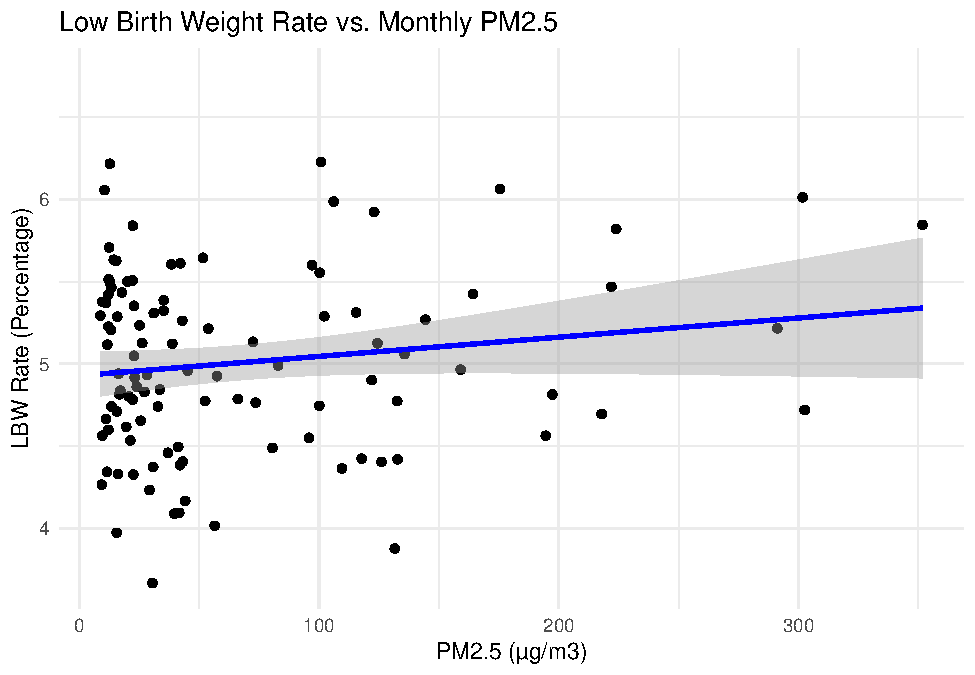
\includegraphics{v_1_files/figure-latex/unnamed-chunk-2-1.pdf} \# Linear
regression

\begin{Shaded}
\begin{Highlighting}[]
\NormalTok{model }\OtherTok{\textless{}{-}} \FunctionTok{lm}\NormalTok{(LBW\_rate }\SpecialCharTok{\textasciitilde{}}\NormalTok{ raw\_conc\_monthly, }\AttributeTok{data =}\NormalTok{ full\_data)}
\FunctionTok{tidy}\NormalTok{(model) }\SpecialCharTok{\%\textgreater{}\%}
  \FunctionTok{kable}\NormalTok{(}\AttributeTok{caption=}\StringTok{"Regression of LBW Rate on PM2.5"}\NormalTok{, }\AttributeTok{digits=}\DecValTok{3}\NormalTok{) }\SpecialCharTok{\%\textgreater{}\%}
  \FunctionTok{kable\_styling}\NormalTok{(}\AttributeTok{full\_width=}\ConstantTok{FALSE}\NormalTok{)}
\end{Highlighting}
\end{Shaded}

\begin{verbatim}
## Warning in attr(x, "align"): 'xfun::attr()' is deprecated.
## Use 'xfun::attr2()' instead.
## See help("Deprecated")
\end{verbatim}

\begin{verbatim}
## Warning in attr(.knitEnv$meta, "knit_meta_id"): 'xfun::attr()' is deprecated.
## Use 'xfun::attr2()' instead.
## See help("Deprecated")
## Warning in attr(.knitEnv$meta, "knit_meta_id"): 'xfun::attr()' is deprecated.
## Use 'xfun::attr2()' instead.
## See help("Deprecated")
## Warning in attr(.knitEnv$meta, "knit_meta_id"): 'xfun::attr()' is deprecated.
## Use 'xfun::attr2()' instead.
## See help("Deprecated")
## Warning in attr(.knitEnv$meta, "knit_meta_id"): 'xfun::attr()' is deprecated.
## Use 'xfun::attr2()' instead.
## See help("Deprecated")
## Warning in attr(.knitEnv$meta, "knit_meta_id"): 'xfun::attr()' is deprecated.
## Use 'xfun::attr2()' instead.
## See help("Deprecated")
## Warning in attr(.knitEnv$meta, "knit_meta_id"): 'xfun::attr()' is deprecated.
## Use 'xfun::attr2()' instead.
## See help("Deprecated")
## Warning in attr(.knitEnv$meta, "knit_meta_id"): 'xfun::attr()' is deprecated.
## Use 'xfun::attr2()' instead.
## See help("Deprecated")
## Warning in attr(.knitEnv$meta, "knit_meta_id"): 'xfun::attr()' is deprecated.
## Use 'xfun::attr2()' instead.
## See help("Deprecated")
## Warning in attr(.knitEnv$meta, "knit_meta_id"): 'xfun::attr()' is deprecated.
## Use 'xfun::attr2()' instead.
## See help("Deprecated")
## Warning in attr(.knitEnv$meta, "knit_meta_id"): 'xfun::attr()' is deprecated.
## Use 'xfun::attr2()' instead.
## See help("Deprecated")
## Warning in attr(.knitEnv$meta, "knit_meta_id"): 'xfun::attr()' is deprecated.
## Use 'xfun::attr2()' instead.
## See help("Deprecated")
## Warning in attr(.knitEnv$meta, "knit_meta_id"): 'xfun::attr()' is deprecated.
## Use 'xfun::attr2()' instead.
## See help("Deprecated")
## Warning in attr(.knitEnv$meta, "knit_meta_id"): 'xfun::attr()' is deprecated.
## Use 'xfun::attr2()' instead.
## See help("Deprecated")
## Warning in attr(.knitEnv$meta, "knit_meta_id"): 'xfun::attr()' is deprecated.
## Use 'xfun::attr2()' instead.
## See help("Deprecated")
\end{verbatim}

\begin{verbatim}
## Warning in attr(x, "align"): 'xfun::attr()' is deprecated.
## Use 'xfun::attr2()' instead.
## See help("Deprecated")
\end{verbatim}

\begin{verbatim}
## Warning in attr(x, "format"): 'xfun::attr()' is deprecated.
## Use 'xfun::attr2()' instead.
## See help("Deprecated")
\end{verbatim}

\begin{longtable}[t]{lrrrr}
\caption{\label{tab:unnamed-chunk-3}Regression of LBW Rate on PM2.5}\\
\toprule
term & estimate & std.error & statistic & p.value\\
\midrule
(Intercept) & 4.928 & 0.072 & 68.089 & 0.000\\
raw\_conc\_monthly & 0.001 & 0.001 & 1.597 & 0.113\\
\bottomrule
\end{longtable}

\begin{Shaded}
\begin{Highlighting}[]
\CommentTok{\# Create proportion of low birth weight}
\NormalTok{full\_data }\OtherTok{\textless{}{-}}\NormalTok{ full\_data }\SpecialCharTok{\%\textgreater{}\%}
  \FunctionTok{mutate}\NormalTok{(}\AttributeTok{Proportion\_LBW =}\NormalTok{ Low\_Birth\_Weight }\SpecialCharTok{/}\NormalTok{ Live\_Births)}
\end{Highlighting}
\end{Shaded}

Exposure timing plays a key role in accurately identifying how air
pollution affects birth outcomes. Our initial analysis showed a weak and
non-significant association between monthly PM2.5 levels and low birth
weight rates (p = 0.113). This limited result probably occurred because
measuring air pollution in the same month as birth ignores the critical
periods during pregnancy when exposure actually affects fetal growth.

To address this issue, we will use lagged regression methods. Lagged
regression aligns PM2.5 exposure data with biologically relevant periods
earlier in pregnancy, specifically during critical developmental windows
like the second and third trimesters. Aligning exposure measurements
with these sensitive gestational periods, similar to optimizing exposure
timing in optical measurement systems (Wang et al., 2020; Li et al.,
2021; Zhang et al., 2019), helps to minimize measurement uncertainty,
reduce confounding from seasonal variations, and accurately identify the
true health impacts of PM2.5 exposure on birth weight outcomes.

References: Li et al., 2021; Wang et al., 2020; Zhang et al., 2019.

\begin{Shaded}
\begin{Highlighting}[]
\CommentTok{\# making sure it\textquotesingle{}s sorted by date}
\NormalTok{full\_data }\OtherTok{\textless{}{-}}\NormalTok{ full\_data }\SpecialCharTok{\%\textgreater{}\%} 
  \FunctionTok{arrange}\NormalTok{(Date)}

\CommentTok{\# creating lags }
\NormalTok{full\_data }\OtherTok{\textless{}{-}}\NormalTok{ full\_data }\SpecialCharTok{\%\textgreater{}\%} 
  \FunctionTok{mutate}\NormalTok{(}
    \AttributeTok{pm25\_lag0 =}\NormalTok{ raw\_conc\_monthly,}
    \AttributeTok{pm25\_lag1 =} \FunctionTok{lag}\NormalTok{(raw\_conc\_monthly, }\DecValTok{1}\NormalTok{),}
    \AttributeTok{pm25\_lag2 =} \FunctionTok{lag}\NormalTok{(raw\_conc\_monthly, }\DecValTok{2}\NormalTok{),}
    \AttributeTok{pm25\_lag3 =} \FunctionTok{lag}\NormalTok{(raw\_conc\_monthly, }\DecValTok{3}\NormalTok{)}
\NormalTok{  )}

\CommentTok{\# fitting a “distributed‐lag” linear model on the LBW rate}
\NormalTok{model\_lag }\OtherTok{\textless{}{-}} \FunctionTok{lm}\NormalTok{(LBW\_rate }\SpecialCharTok{\textasciitilde{}}\NormalTok{ pm25\_lag0 }\SpecialCharTok{+}\NormalTok{ pm25\_lag1 }\SpecialCharTok{+}\NormalTok{ pm25\_lag2 }\SpecialCharTok{+}\NormalTok{ pm25\_lag3,}
                \AttributeTok{data =}\NormalTok{ full\_data)}

\CommentTok{\# inspecting the month‐specific coefficients}
\FunctionTok{tidy}\NormalTok{(model\_lag) }\SpecialCharTok{\%\textgreater{}\%} 
  \FunctionTok{kable}\NormalTok{(}\AttributeTok{digits=}\DecValTok{3}\NormalTok{, }\AttributeTok{caption=}\StringTok{"Lagged PM 2.5 Effects on LBW Rate"}\NormalTok{) }\SpecialCharTok{\%\textgreater{}\%}
  \FunctionTok{kable\_styling}\NormalTok{(}\AttributeTok{full\_width=}\ConstantTok{FALSE}\NormalTok{)}
\end{Highlighting}
\end{Shaded}

\begin{verbatim}
## Warning in attr(x, "align"): 'xfun::attr()' is deprecated.
## Use 'xfun::attr2()' instead.
## See help("Deprecated")
\end{verbatim}

\begin{verbatim}
## Warning in attr(.knitEnv$meta, "knit_meta_id"): 'xfun::attr()' is deprecated.
## Use 'xfun::attr2()' instead.
## See help("Deprecated")
## Warning in attr(.knitEnv$meta, "knit_meta_id"): 'xfun::attr()' is deprecated.
## Use 'xfun::attr2()' instead.
## See help("Deprecated")
## Warning in attr(.knitEnv$meta, "knit_meta_id"): 'xfun::attr()' is deprecated.
## Use 'xfun::attr2()' instead.
## See help("Deprecated")
## Warning in attr(.knitEnv$meta, "knit_meta_id"): 'xfun::attr()' is deprecated.
## Use 'xfun::attr2()' instead.
## See help("Deprecated")
## Warning in attr(.knitEnv$meta, "knit_meta_id"): 'xfun::attr()' is deprecated.
## Use 'xfun::attr2()' instead.
## See help("Deprecated")
## Warning in attr(.knitEnv$meta, "knit_meta_id"): 'xfun::attr()' is deprecated.
## Use 'xfun::attr2()' instead.
## See help("Deprecated")
## Warning in attr(.knitEnv$meta, "knit_meta_id"): 'xfun::attr()' is deprecated.
## Use 'xfun::attr2()' instead.
## See help("Deprecated")
## Warning in attr(.knitEnv$meta, "knit_meta_id"): 'xfun::attr()' is deprecated.
## Use 'xfun::attr2()' instead.
## See help("Deprecated")
## Warning in attr(.knitEnv$meta, "knit_meta_id"): 'xfun::attr()' is deprecated.
## Use 'xfun::attr2()' instead.
## See help("Deprecated")
## Warning in attr(.knitEnv$meta, "knit_meta_id"): 'xfun::attr()' is deprecated.
## Use 'xfun::attr2()' instead.
## See help("Deprecated")
## Warning in attr(.knitEnv$meta, "knit_meta_id"): 'xfun::attr()' is deprecated.
## Use 'xfun::attr2()' instead.
## See help("Deprecated")
## Warning in attr(.knitEnv$meta, "knit_meta_id"): 'xfun::attr()' is deprecated.
## Use 'xfun::attr2()' instead.
## See help("Deprecated")
## Warning in attr(.knitEnv$meta, "knit_meta_id"): 'xfun::attr()' is deprecated.
## Use 'xfun::attr2()' instead.
## See help("Deprecated")
## Warning in attr(.knitEnv$meta, "knit_meta_id"): 'xfun::attr()' is deprecated.
## Use 'xfun::attr2()' instead.
## See help("Deprecated")
\end{verbatim}

\begin{verbatim}
## Warning in attr(x, "align"): 'xfun::attr()' is deprecated.
## Use 'xfun::attr2()' instead.
## See help("Deprecated")
\end{verbatim}

\begin{verbatim}
## Warning in attr(x, "format"): 'xfun::attr()' is deprecated.
## Use 'xfun::attr2()' instead.
## See help("Deprecated")
\end{verbatim}

\begin{longtable}[t]{lrrrr}
\caption{\label{tab:unnamed-chunk-4}Lagged PM 2.5 Effects on LBW Rate}\\
\toprule
term & estimate & std.error & statistic & p.value\\
\midrule
(Intercept) & 5.053 & 0.097 & 52.155 & 0.000\\
pm25\_lag0 & -0.001 & 0.002 & -0.369 & 0.713\\
pm25\_lag1 & 0.002 & 0.003 & 0.750 & 0.455\\
pm25\_lag2 & 0.001 & 0.003 & 0.441 & 0.660\\
pm25\_lag3 & -0.003 & 0.002 & -1.742 & 0.085\\
\bottomrule
\end{longtable}

\begin{Shaded}
\begin{Highlighting}[]
\CommentTok{\# \# Check correlations}
\FunctionTok{cor}\NormalTok{(full\_data }\SpecialCharTok{\%\textgreater{}\%} \FunctionTok{select}\NormalTok{(pm25\_lag0}\SpecialCharTok{:}\NormalTok{pm25\_lag3), }\AttributeTok{use =} \StringTok{"pairwise.complete.obs"}\NormalTok{)}
\end{Highlighting}
\end{Shaded}

\begin{verbatim}
##             pm25_lag0 pm25_lag1 pm25_lag2   pm25_lag3
## pm25_lag0  1.00000000 0.7976814 0.3524914 -0.08144454
## pm25_lag1  0.79768139 1.0000000 0.7976814  0.35249139
## pm25_lag2  0.35249139 0.7976814 1.0000000  0.80600809
## pm25_lag3 -0.08144454 0.3524914 0.8060081  1.00000000
\end{verbatim}

\begin{Shaded}
\begin{Highlighting}[]
\CommentTok{\# Or VIFs}
\FunctionTok{library}\NormalTok{(car)}
\end{Highlighting}
\end{Shaded}

\begin{verbatim}
## Loading required package: carData
\end{verbatim}

\begin{verbatim}
## 
## Attaching package: 'car'
\end{verbatim}

\begin{verbatim}
## The following object is masked from 'package:dplyr':
## 
##     recode
\end{verbatim}

\begin{verbatim}
## The following object is masked from 'package:purrr':
## 
##     some
\end{verbatim}

\begin{Shaded}
\begin{Highlighting}[]
\FunctionTok{vif}\NormalTok{(}\FunctionTok{lm}\NormalTok{(LBW\_rate }\SpecialCharTok{\textasciitilde{}}\NormalTok{ pm25\_lag0 }\SpecialCharTok{+}\NormalTok{ pm25\_lag1 }\SpecialCharTok{+}\NormalTok{ pm25\_lag2 }\SpecialCharTok{+}\NormalTok{ pm25\_lag3,}
       \AttributeTok{data =}\NormalTok{ full\_data))}
\end{Highlighting}
\end{Shaded}

\begin{verbatim}
## pm25_lag0 pm25_lag1 pm25_lag2 pm25_lag3 
##  4.059541  8.888158  8.078684  3.442012
\end{verbatim}

\begin{Shaded}
\begin{Highlighting}[]
\CommentTok{\# Cumulative two‐month average}
\NormalTok{full\_data }\OtherTok{\textless{}{-}}\NormalTok{ full\_data }\SpecialCharTok{\%\textgreater{}\%}
  \FunctionTok{mutate}\NormalTok{(}\AttributeTok{pm25\_cum23 =}\NormalTok{ (pm25\_lag2 }\SpecialCharTok{+}\NormalTok{ pm25\_lag3) }\SpecialCharTok{/} \DecValTok{2}\NormalTok{)}

\FunctionTok{lm}\NormalTok{(LBW\_rate }\SpecialCharTok{\textasciitilde{}}\NormalTok{ pm25\_cum23, }\AttributeTok{data =}\NormalTok{ full\_data) }\SpecialCharTok{\%\textgreater{}\%}\NormalTok{ broom}\SpecialCharTok{::}\FunctionTok{tidy}\NormalTok{()}
\end{Highlighting}
\end{Shaded}

\begin{verbatim}
## # A tibble: 2 x 5
##   term         estimate std.error statistic  p.value
##   <chr>           <dbl>     <dbl>     <dbl>    <dbl>
## 1 (Intercept)  5.06      0.0803      63.0   6.68e-83
## 2 pm25_cum23  -0.000219  0.000885    -0.248 8.05e- 1
\end{verbatim}

\begin{Shaded}
\begin{Highlighting}[]
\NormalTok{dlm }\OtherTok{\textless{}{-}} \FunctionTok{lm}\NormalTok{(LBW\_rate }\SpecialCharTok{\textasciitilde{}}\NormalTok{ pm25\_lag0 }\SpecialCharTok{+}\NormalTok{ pm25\_lag1 }\SpecialCharTok{+}\NormalTok{ pm25\_lag2 }\SpecialCharTok{+}\NormalTok{ pm25\_lag3,}
          \AttributeTok{data =}\NormalTok{ full\_data)}
\FunctionTok{linearHypothesis}\NormalTok{(dlm, }\FunctionTok{c}\NormalTok{(}\StringTok{"pm25\_lag0 = 0"}\NormalTok{,}
                        \StringTok{"pm25\_lag1 = 0"}\NormalTok{,}
                        \StringTok{"pm25\_lag2 = 0"}\NormalTok{,}
                        \StringTok{"pm25\_lag3 = 0"}\NormalTok{))}
\end{Highlighting}
\end{Shaded}

\begin{verbatim}
## 
## Linear hypothesis test:
## pm25_lag0 = 0
## pm25_lag1 = 0
## pm25_lag2 = 0
## pm25_lag3 = 0
## 
## Model 1: restricted model
## Model 2: LBW_rate ~ pm25_lag0 + pm25_lag1 + pm25_lag2 + pm25_lag3
## 
##   Res.Df    RSS Df Sum of Sq      F  Pr(>F)  
## 1     97 30.650                              
## 2     93 28.169  4    2.4807 2.0475 0.09408 .
## ---
## Signif. codes:  0 '***' 0.001 '**' 0.01 '*' 0.05 '.' 0.1 ' ' 1
\end{verbatim}

\begin{Shaded}
\begin{Highlighting}[]
\DocumentationTok{\#\# Collapse to 2{-} and 3{-}month cumulative PM 2.5 averages and re{-}fit}

\FunctionTok{library}\NormalTok{(dplyr)}
\FunctionTok{library}\NormalTok{(broom)}
\FunctionTok{library}\NormalTok{(knitr)}
\FunctionTok{library}\NormalTok{(kableExtra)}

\CommentTok{\# 1) Create cumulative exposure variables}
\NormalTok{full\_data }\OtherTok{\textless{}{-}}\NormalTok{ full\_data }\SpecialCharTok{\%\textgreater{}\%}
  \FunctionTok{arrange}\NormalTok{(Date) }\SpecialCharTok{\%\textgreater{}\%}
  \FunctionTok{mutate}\NormalTok{(}
    \AttributeTok{pm25\_cum12  =}\NormalTok{ (pm25\_lag1 }\SpecialCharTok{+}\NormalTok{ pm25\_lag2) }\SpecialCharTok{/} \DecValTok{2}\NormalTok{,          }\CommentTok{\# average of 1{-} and 2{-}month lags}
    \AttributeTok{pm25\_cum123 =}\NormalTok{ (pm25\_lag1 }\SpecialCharTok{+}\NormalTok{ pm25\_lag2 }\SpecialCharTok{+}\NormalTok{ pm25\_lag3) }\SpecialCharTok{/} \DecValTok{3}  \CommentTok{\# average of 1{-}, 2{-}, 3{-}month lags}
\NormalTok{  )}

\CommentTok{\# 2) Fit separate linear models}
\NormalTok{model\_cum12  }\OtherTok{\textless{}{-}} \FunctionTok{lm}\NormalTok{(LBW\_rate }\SpecialCharTok{\textasciitilde{}}\NormalTok{ pm25\_cum12,  }\AttributeTok{data =}\NormalTok{ full\_data)}
\NormalTok{model\_cum123 }\OtherTok{\textless{}{-}} \FunctionTok{lm}\NormalTok{(LBW\_rate }\SpecialCharTok{\textasciitilde{}}\NormalTok{ pm25\_cum123, }\AttributeTok{data =}\NormalTok{ full\_data)}

\CommentTok{\# 3) Summarize and display results side by side}
\NormalTok{results }\OtherTok{\textless{}{-}} \FunctionTok{bind\_rows}\NormalTok{(}
  \FunctionTok{tidy}\NormalTok{(model\_cum12)  }\SpecialCharTok{\%\textgreater{}\%} \FunctionTok{mutate}\NormalTok{(}\AttributeTok{model =} \StringTok{"cum12"}\NormalTok{),}
  \FunctionTok{tidy}\NormalTok{(model\_cum123) }\SpecialCharTok{\%\textgreater{}\%} \FunctionTok{mutate}\NormalTok{(}\AttributeTok{model =} \StringTok{"cum123"}\NormalTok{)}
\NormalTok{) }\SpecialCharTok{\%\textgreater{}\%}
  \FunctionTok{select}\NormalTok{(model, term, estimate, std.error, statistic, p.value)}

\NormalTok{results }\SpecialCharTok{\%\textgreater{}\%}
  \FunctionTok{kable}\NormalTok{(}
    \AttributeTok{caption =} \StringTok{"Regression of LBW Rate on Cumulative PM2.5 Averages"}\NormalTok{,}
    \AttributeTok{digits  =} \DecValTok{3}
\NormalTok{  ) }\SpecialCharTok{\%\textgreater{}\%}
  \FunctionTok{kable\_styling}\NormalTok{(}\AttributeTok{full\_width =} \ConstantTok{FALSE}\NormalTok{)}
\end{Highlighting}
\end{Shaded}

\begin{verbatim}
## Warning in attr(x, "align"): 'xfun::attr()' is deprecated.
## Use 'xfun::attr2()' instead.
## See help("Deprecated")
\end{verbatim}

\begin{verbatim}
## Warning in attr(.knitEnv$meta, "knit_meta_id"): 'xfun::attr()' is deprecated.
## Use 'xfun::attr2()' instead.
## See help("Deprecated")
## Warning in attr(.knitEnv$meta, "knit_meta_id"): 'xfun::attr()' is deprecated.
## Use 'xfun::attr2()' instead.
## See help("Deprecated")
## Warning in attr(.knitEnv$meta, "knit_meta_id"): 'xfun::attr()' is deprecated.
## Use 'xfun::attr2()' instead.
## See help("Deprecated")
## Warning in attr(.knitEnv$meta, "knit_meta_id"): 'xfun::attr()' is deprecated.
## Use 'xfun::attr2()' instead.
## See help("Deprecated")
## Warning in attr(.knitEnv$meta, "knit_meta_id"): 'xfun::attr()' is deprecated.
## Use 'xfun::attr2()' instead.
## See help("Deprecated")
## Warning in attr(.knitEnv$meta, "knit_meta_id"): 'xfun::attr()' is deprecated.
## Use 'xfun::attr2()' instead.
## See help("Deprecated")
## Warning in attr(.knitEnv$meta, "knit_meta_id"): 'xfun::attr()' is deprecated.
## Use 'xfun::attr2()' instead.
## See help("Deprecated")
## Warning in attr(.knitEnv$meta, "knit_meta_id"): 'xfun::attr()' is deprecated.
## Use 'xfun::attr2()' instead.
## See help("Deprecated")
## Warning in attr(.knitEnv$meta, "knit_meta_id"): 'xfun::attr()' is deprecated.
## Use 'xfun::attr2()' instead.
## See help("Deprecated")
## Warning in attr(.knitEnv$meta, "knit_meta_id"): 'xfun::attr()' is deprecated.
## Use 'xfun::attr2()' instead.
## See help("Deprecated")
## Warning in attr(.knitEnv$meta, "knit_meta_id"): 'xfun::attr()' is deprecated.
## Use 'xfun::attr2()' instead.
## See help("Deprecated")
## Warning in attr(.knitEnv$meta, "knit_meta_id"): 'xfun::attr()' is deprecated.
## Use 'xfun::attr2()' instead.
## See help("Deprecated")
## Warning in attr(.knitEnv$meta, "knit_meta_id"): 'xfun::attr()' is deprecated.
## Use 'xfun::attr2()' instead.
## See help("Deprecated")
## Warning in attr(.knitEnv$meta, "knit_meta_id"): 'xfun::attr()' is deprecated.
## Use 'xfun::attr2()' instead.
## See help("Deprecated")
\end{verbatim}

\begin{verbatim}
## Warning in attr(x, "align"): 'xfun::attr()' is deprecated.
## Use 'xfun::attr2()' instead.
## See help("Deprecated")
\end{verbatim}

\begin{verbatim}
## Warning in attr(x, "format"): 'xfun::attr()' is deprecated.
## Use 'xfun::attr2()' instead.
## See help("Deprecated")
\end{verbatim}

\begin{longtable}[t]{llrrrr}
\caption{\label{tab:unnamed-chunk-4}Regression of LBW Rate on Cumulative PM2.5 Averages}\\
\toprule
model & term & estimate & std.error & statistic & p.value\\
\midrule
cum12 & (Intercept) & 4.944 & 0.080 & 62.183 & 0.000\\
cum12 & pm25\_cum12 & 0.001 & 0.001 & 1.421 & 0.158\\
cum123 & (Intercept) & 4.985 & 0.085 & 58.483 & 0.000\\
cum123 & pm25\_cum123 & 0.001 & 0.001 & 0.863 & 0.390\\
\bottomrule
\end{longtable}

\begin{Shaded}
\begin{Highlighting}[]
\CommentTok{\#install.packages("dlnm")}
\FunctionTok{library}\NormalTok{(dlnm)}
\end{Highlighting}
\end{Shaded}

\begin{verbatim}
## This is dlnm 2.4.10. For details: help(dlnm) and vignette('dlnmOverview').
\end{verbatim}

\begin{Shaded}
\begin{Highlighting}[]
\CommentTok{\# cross{-}basis for a 6{-}month lag window}
\FunctionTok{library}\NormalTok{(dlnm)}

\CommentTok{\# 1. define a cross‐basis for raw\_conc\_monthly up to 3‐month lag}
\NormalTok{cb }\OtherTok{\textless{}{-}} \FunctionTok{crossbasis}\NormalTok{(}
\NormalTok{  full\_data}\SpecialCharTok{$}\NormalTok{raw\_conc\_monthly,}
  \AttributeTok{lag     =} \DecValTok{3}\NormalTok{,}
  \AttributeTok{argvar  =} \FunctionTok{list}\NormalTok{(}\AttributeTok{fun=}\StringTok{"ns"}\NormalTok{, }\AttributeTok{df=}\DecValTok{3}\NormalTok{),   }\CommentTok{\# natural spline on the exposure–response}
  \AttributeTok{arglag  =} \FunctionTok{list}\NormalTok{(}\AttributeTok{fun=}\StringTok{"ns"}\NormalTok{, }\AttributeTok{df=}\DecValTok{3}\NormalTok{)    }\CommentTok{\# natural spline on the lag–response}
\NormalTok{)}

\CommentTok{\# 2. fit the model *including* cb, not the separate pm25\_lag0… variables}
\NormalTok{dlmod }\OtherTok{\textless{}{-}} \FunctionTok{lm}\NormalTok{(LBW\_rate }\SpecialCharTok{\textasciitilde{}}\NormalTok{ cb, }\AttributeTok{data =}\NormalTok{ full\_data)}


\NormalTok{cen\_pm25 }\OtherTok{\textless{}{-}} \FunctionTok{median}\NormalTok{(full\_data}\SpecialCharTok{$}\NormalTok{raw\_conc\_monthly, }\AttributeTok{na.rm=}\ConstantTok{TRUE}\NormalTok{)}

\NormalTok{pred }\OtherTok{\textless{}{-}} \FunctionTok{crosspred}\NormalTok{(}
\NormalTok{  cb,            }\CommentTok{\# your crossbasis}
\NormalTok{  dlmod,         }\CommentTok{\# your dlm with cb in it}
  \AttributeTok{at   =}\NormalTok{ cen\_pm25,}
  \AttributeTok{cen  =}\NormalTok{ cen\_pm25,}
  \AttributeTok{bylag =} \DecValTok{1}
\NormalTok{)}


\CommentTok{\# now draw the lag‐response curve:}
\FunctionTok{plot}\NormalTok{(}
\NormalTok{  pred,}
  \StringTok{"slices"}\NormalTok{,           }\CommentTok{\# draw slices}
  \AttributeTok{var   =}\NormalTok{ cen\_pm25,   }\CommentTok{\# which PM2.5 to slice at}
  \AttributeTok{ci    =} \StringTok{"lines"}\NormalTok{,    }\CommentTok{\# draw the 95\% CI as lines}
  \AttributeTok{xlab  =} \StringTok{"Lag (months)"}\NormalTok{,}
  \AttributeTok{ylab  =} \StringTok{"Change in LBW rate (Percantage)"}\NormalTok{,}
  \AttributeTok{main  =} \FunctionTok{paste0}\NormalTok{(}
    \StringTok{"Lag–response at PM2.5 = "}\NormalTok{, }
    \FunctionTok{round}\NormalTok{(cen\_pm25,}\DecValTok{1}\NormalTok{), }
    \StringTok{" µg/m3"}
\NormalTok{  )}
\NormalTok{)}
\end{Highlighting}
\end{Shaded}

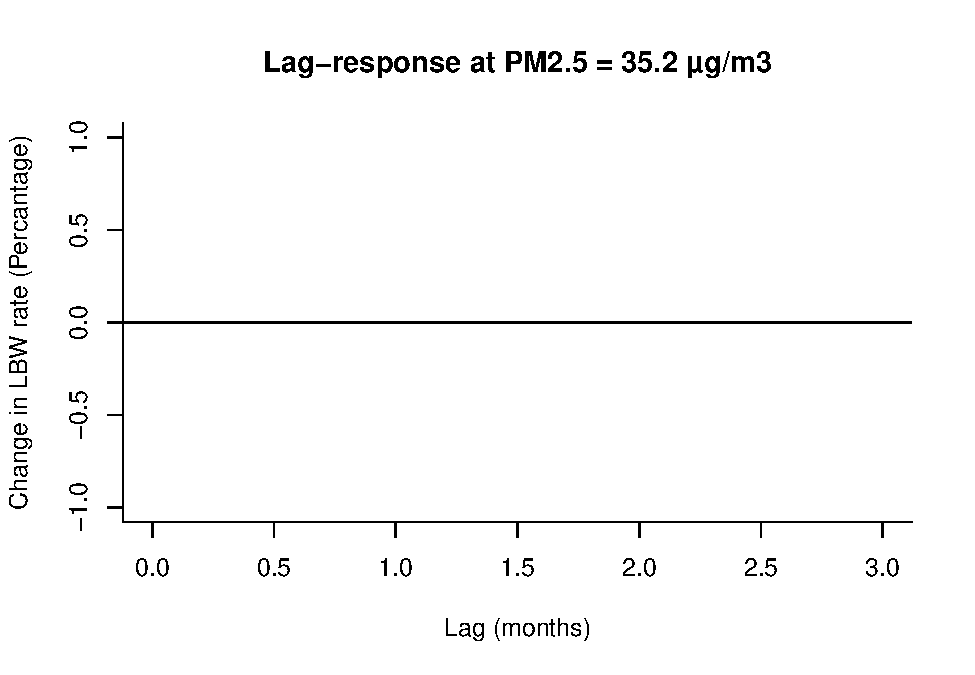
\includegraphics{v_1_files/figure-latex/unnamed-chunk-5-1.pdf}

\begin{center}\rule{0.5\linewidth}{0.5pt}\end{center}

\section{End of Analysis}\label{end-of-analysis}

\end{document}
